\documentclass[12pt, twoside]{article}
\usepackage[letterpaper, margin=1in, headsep=0.5in]{geometry}
\usepackage[english]{babel}
\usepackage[utf8]{inputenc}
\usepackage{amsmath}
\usepackage{amsfonts}
\usepackage{amssymb}
\usepackage{tikz}
%\usetikzlibrary{quotes, angles}

\usepackage{graphicx}
\usepackage{enumitem}
\usepackage{multicol}

\usepackage{fancyhdr}
\pagestyle{fancy}
\fancyhf{}
\renewcommand{\headrulewidth}{0pt} % disable the underline of the header

\fancyhead[RE]{\thepage}
\fancyhead[RO]{\thepage \\ Name: \hspace{3cm}}
\fancyhead[L]{BECA / Dr. Huson / 11.1 IB Math SL\\*
Test: Exponential and logarithmic functions\\* 13 December 2018}

\begin{document}
\textit{Answer separately on lined paper unless otherwise instructed.}
\subsubsection*{Part 1: No calculators are allowed on this section.}

Simplify. Leave no negative or fractional exponents.

\begin{enumerate}

\item $15x^{2}y^2 \div 3x^5 y^{2}$
\item $\sqrt[3]{x^{-9} y^{6}}$
\item $\displaystyle \left( x y^{\frac{1}{4}}\right)^2$
\item $\log_5 25$
\item $\log_6 4 + \log_6 9$
\item $\log 200 - \log 2$
\item $(x-3)(x^2+3x+9)$

\item The diagram below shows the graph of a function $f$, composed of four points.
  \begin{center}
  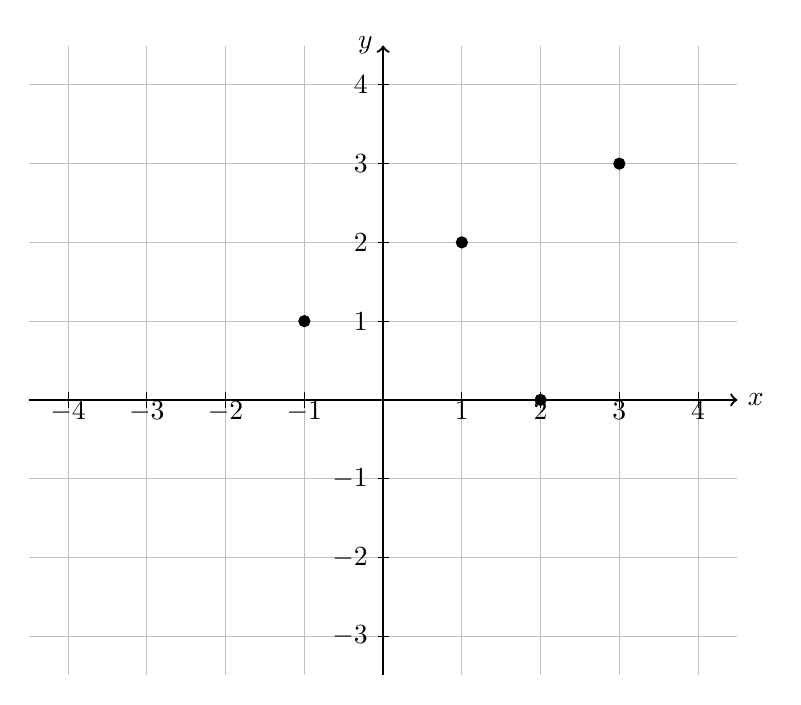
\begin{tikzpicture}
      %grid
      \draw [thin, color=lightgray,, xstep=1.0cm,ystep=1.0cm] (-4.5,-3.5) grid (4.5,4.5);
      %\draw [thin, color=lightgray,, xstep=0.2cm,ystep=0.2cm] (-4.5,-1.5) grid (5.5,16.5);

      \foreach \x in {-4, -3, -2, -1,1,2,3,4}
      \draw[shift={(\x,0)},color=black] (0pt,-3pt) -- (0pt,3pt) node[below]  {$\x$};

      \foreach \y in {-3, -2, -1, 1,2,3,4}
      \draw[shift={(0,\y)},color=black] (2pt,0pt) -- (-2pt,0pt) node[left]  {$\y$};

      \draw [thick, ->] (-4.5,0) -- (+4.5,0) node [right] {$x$};
      \draw [thick, ->] (0,-3.5) -- (0,4.5) node [left] {$y$};

      \draw [fill](3,3) circle[radius=2pt];
      \draw [fill](2,0) circle[radius=2pt];
      \draw [fill](1,2) circle[radius=2pt];
      \draw [fill](-1,1) circle[radius=2pt];
      %\draw plot[domain= -1:3] (\x, (\x+1)*(\x+1) - 4);
  \end{tikzpicture}
  \end{center}

\begin{enumerate}
    \item Write down the value of $f(2)$.
    \item Write down the domain of $f$.
    \item Write down the range of $f$.
    \item Write down the value of $f^{-1}(1)$.
    \item Sketch the inverse of $f$, $f^{-1}$, on the grid above.
\end{enumerate}

\newpage

\item Let $f(x)=3x-1$ and $g(x)=-2x^2+2$
\begin{enumerate}
    \item Find $f^{-1}(x)$.
    \item Find $(f \circ g)(1)$.
\end{enumerate}

\item Consider the equation $x^2 + (k-2)x=-4$, where $k$ is a real number. Find the values of $k$ for which the equation has two equal real solutions.

\item Let $f$ be a quadratic function. Part of the graph of $f$ is shown below.\\*
The vertex is at $P(2,1)$ and the $y$-intercept is at $Q(0, 3)$.\\*

  \begin{figure}[!htbp]
  \begin{center}
  \begin{tikzpicture}

      %grid
      %\draw [thin, color=lightgray,, xstep=1.0cm,ystep=1.0cm] (-5.5,-5.5) grid (5.5,5.5);
      %\draw [thin, color=lightgray,, xstep=0.2cm,ystep=0.2cm] (-5.5,-1.5) grid (5.5,16.5);

      \foreach \x in {-2, -1,1,2,3,4,5,6}
      \draw[shift={(\x,0)},color=black] (0pt,-3pt) -- (0pt,3pt) node[below]  {$\x$};

      \foreach \y in {-1,1,2,3,4,5,6}
      \draw[shift={(0,\y)},color=black] (2pt,0pt) -- (-2pt,0pt) node[left]  {$\y$};

      \draw [thick, ->] (-2.5,0) -- (+6.5,0) node [right] {$x$};
      \draw [thick, ->] (0,-1.5) -- (0,6.5) node [left] {$y$};

      \draw [fill] (1,2) circle[radius=2pt] node [below] {$P$};
      \draw [fill] (0,4) circle[radius=2pt] node [right] {$Q$};

      \draw [<->] plot[domain= -0.5:2.5] (\x, 2*\x*\x -4*\x +4);

  \end{tikzpicture}
  \end{center}
  \end{figure}

\begin{enumerate}
    \item Write down the equation of the axis of symmetry.
    \item The function $f$ can be written in the form $f(x)=a(x-h)^2 +k$. \\*
    Write down the value of $h$ and of $k$.
    \item Find $a$.
\end{enumerate}

\newpage
\subsubsection*{Part 2: Graphing calculators may be used on this section.}

\item Let $f(x)=3x^2-12x+7$.
\begin{enumerate}
    \item Write down the coordinates of the vertex.
    \item Hence or otherwise, express the function in the form $f(x)=3(x-h)^2 +k$.
    \item Solve the equation  $f(x)=0$.
\end{enumerate}

\item Paulita takes medication. After $t$ minutes, the concentration of medication left in her bloodstream is given by $\displaystyle C(t)=15(0.5)^{(0.02t)}$, where $C$ is in milligrams per litre.
\begin{enumerate}
    \item Write down $C(0)$.
    \item Find the concentration of medication left in her bloodstream after 25 minutes.
    \item At 8:00, when there is no medication in Paulita's bloodstream, she takes her first dose of medication. She can take her medication again when the concentration of medication reaches 3.00 milligrams per litre. What time will Paulita be able to take her medication again?
\end{enumerate}

\item A student takes out a loan for \$8,000 to cover college expenses. Interest of 7\% per annum is charged, compounded monthly. Use the interest rate formula \[P(t)=P_0(1+\frac{r}{n})^{nt}\] where $P(t)$ is the total interest and principal at time $t$, $P_0$ is the initial loan amount, $t$ is the time in years, $r=7\%$ is the interest rate per annum, and $n=12$ is the number of compounding periods per year.
\begin{enumerate}
  \item Calculate how much she will owe after five years, \emph{rounded to the nearest dollar}.
  \item How long will it take for the outstanding balance to double, \emph{to the nearest month}?
  \item Spicy: Use an algebraic method to solve the previous question (the time to double).
\end{enumerate}

\newpage
\item Consider the function $f(x)=x^2+2x-2$.
\begin{enumerate}
    \item Sketch the graph of $f$, for $-4 \leq x \leq 2$.
    \item This function can also be written in the form $f(x)=(x-p)^2 -3$.\\*
    Write down the value of $p$.
    \item The graph of $g$ is obtained by reflecting the graph of $f$ in the $x$-axis, followed by a translation of $(0, 2)$.\\* Show that $g(x)=-x^2-2x+4$.
    \item The graphs of $f$ and $g$ intersect at two points.\\*
    Write down the x-coordinates of these two points.
\end{enumerate}

\begin{figure}[!htbp]
\begin{center}
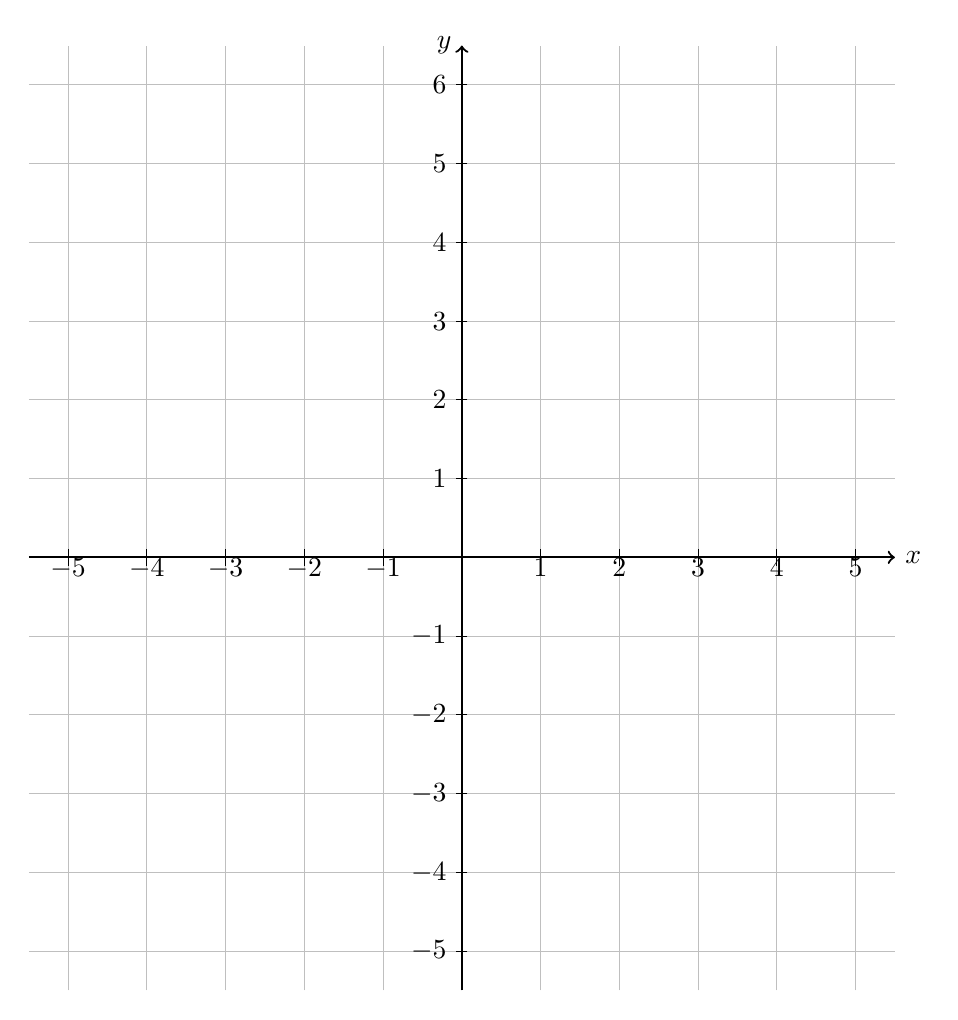
\begin{tikzpicture}

    %grid
    \draw [thin, color=lightgray,, xstep=1.0cm,ystep=1.0cm] (-5.5,-5.5) grid (5.5,6.5);
    %\draw [thin, color=lightgray,, xstep=0.2cm,ystep=0.2cm] (-4.5,-1.5) grid (5.5,16.5);

    \foreach \x in {-5, -4, -3, -2, -1,1,2,3,4, 5}
    \draw[shift={(\x,0)},color=black] (0pt,-3pt) -- (0pt,3pt) node[below]  {$\x$};

    \foreach \y in {-5, -4, -3, -2, -1, 1,2,3,4, 5, 6}
    \draw[shift={(0,\y)},color=black] (2pt,0pt) -- (-2pt,0pt) node[left]  {$\y$};

    \draw [thick, ->] (-5.5,0) -- (+5.5,0) node [right] {$x$};
    \draw [thick, ->] (0,-5.5) -- (0,6.5) node [left] {$y$};

    %\draw plot[domain= -4:2] (\x, (\x*\x +2*\x-2);

\end{tikzpicture}
\end{center}
\end{figure}


\end{enumerate}
\end{document}
